% Created by tikzDevice version 0.10.1 on 2017-11-19 19:19:55
% !TEX encoding = UTF-8 Unicode
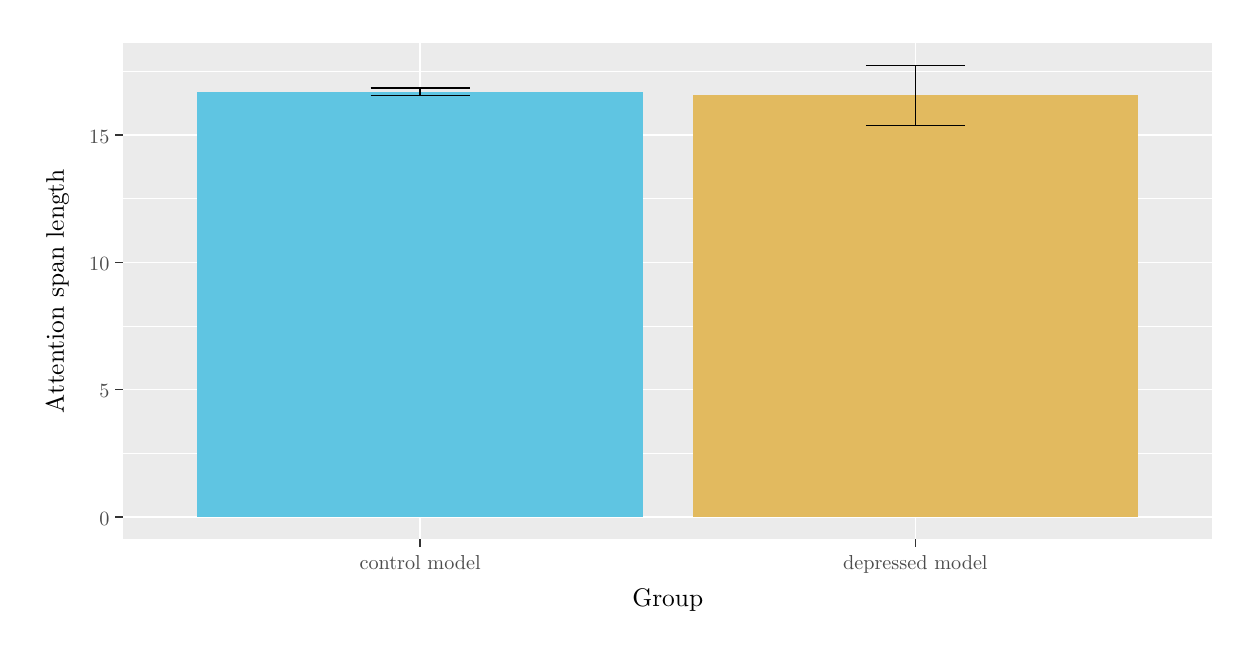
\begin{tikzpicture}[x=1pt,y=1pt]
\definecolor{fillColor}{RGB}{255,255,255}
\path[use as bounding box,fill=fillColor,fill opacity=0.00] (0,0) rectangle (433.62,216.81);
\begin{scope}
\path[clip] (  0.00,  0.00) rectangle (433.62,216.81);
\definecolor{drawColor}{RGB}{255,255,255}
\definecolor{fillColor}{RGB}{255,255,255}

\path[draw=drawColor,line width= 0.6pt,line join=round,line cap=round,fill=fillColor] (  0.00,  0.00) rectangle (433.62,216.81);
\end{scope}
\begin{scope}
\path[clip] ( 34.47, 31.92) rectangle (428.12,211.31);
\definecolor{fillColor}{gray}{0.92}

\path[fill=fillColor] ( 34.47, 31.92) rectangle (428.12,211.31);
\definecolor{drawColor}{RGB}{255,255,255}

\path[draw=drawColor,line width= 0.3pt,line join=round] ( 34.47, 63.06) --
	(428.12, 63.06);

\path[draw=drawColor,line width= 0.3pt,line join=round] ( 34.47,109.02) --
	(428.12,109.02);

\path[draw=drawColor,line width= 0.3pt,line join=round] ( 34.47,154.98) --
	(428.12,154.98);

\path[draw=drawColor,line width= 0.3pt,line join=round] ( 34.47,200.95) --
	(428.12,200.95);

\path[draw=drawColor,line width= 0.6pt,line join=round] ( 34.47, 40.07) --
	(428.12, 40.07);

\path[draw=drawColor,line width= 0.6pt,line join=round] ( 34.47, 86.04) --
	(428.12, 86.04);

\path[draw=drawColor,line width= 0.6pt,line join=round] ( 34.47,132.00) --
	(428.12,132.00);

\path[draw=drawColor,line width= 0.6pt,line join=round] ( 34.47,177.96) --
	(428.12,177.96);

\path[draw=drawColor,line width= 0.6pt,line join=round] (141.83, 31.92) --
	(141.83,211.31);

\path[draw=drawColor,line width= 0.6pt,line join=round] (320.76, 31.92) --
	(320.76,211.31);
\definecolor{fillColor}{RGB}{95,197,226}

\path[fill=fillColor] ( 61.31, 40.07) rectangle (222.35,193.63);
\definecolor{fillColor}{RGB}{226,186,95}

\path[fill=fillColor] (240.24, 40.07) rectangle (401.28,192.33);
\definecolor{drawColor}{RGB}{0,0,0}

\path[draw=drawColor,line width= 0.6pt,line join=round] (123.94,194.99) --
	(159.72,194.99);

\path[draw=drawColor,line width= 0.6pt,line join=round] (141.83,194.99) --
	(141.83,192.28);

\path[draw=drawColor,line width= 0.6pt,line join=round] (123.94,192.28) --
	(159.72,192.28);

\path[draw=drawColor,line width= 0.6pt,line join=round] (302.87,203.16) --
	(338.65,203.16);

\path[draw=drawColor,line width= 0.6pt,line join=round] (320.76,203.16) --
	(320.76,181.50);

\path[draw=drawColor,line width= 0.6pt,line join=round] (302.87,181.50) --
	(338.65,181.50);
\end{scope}
\begin{scope}
\path[clip] (  0.00,  0.00) rectangle (433.62,216.81);
\definecolor{drawColor}{gray}{0.30}

\node[text=drawColor,anchor=base east,inner sep=0pt, outer sep=0pt, scale=  0.73] at ( 29.52, 37.04) {0};

\node[text=drawColor,anchor=base east,inner sep=0pt, outer sep=0pt, scale=  0.73] at ( 29.52, 83.01) {5};

\node[text=drawColor,anchor=base east,inner sep=0pt, outer sep=0pt, scale=  0.73] at ( 29.52,128.97) {10};

\node[text=drawColor,anchor=base east,inner sep=0pt, outer sep=0pt, scale=  0.73] at ( 29.52,174.93) {15};
\end{scope}
\begin{scope}
\path[clip] (  0.00,  0.00) rectangle (433.62,216.81);
\definecolor{drawColor}{gray}{0.20}

\path[draw=drawColor,line width= 0.6pt,line join=round] ( 31.72, 40.07) --
	( 34.47, 40.07);

\path[draw=drawColor,line width= 0.6pt,line join=round] ( 31.72, 86.04) --
	( 34.47, 86.04);

\path[draw=drawColor,line width= 0.6pt,line join=round] ( 31.72,132.00) --
	( 34.47,132.00);

\path[draw=drawColor,line width= 0.6pt,line join=round] ( 31.72,177.96) --
	( 34.47,177.96);
\end{scope}
\begin{scope}
\path[clip] (  0.00,  0.00) rectangle (433.62,216.81);
\definecolor{drawColor}{gray}{0.20}

\path[draw=drawColor,line width= 0.6pt,line join=round] (141.83, 29.17) --
	(141.83, 31.92);

\path[draw=drawColor,line width= 0.6pt,line join=round] (320.76, 29.17) --
	(320.76, 31.92);
\end{scope}
\begin{scope}
\path[clip] (  0.00,  0.00) rectangle (433.62,216.81);
\definecolor{drawColor}{gray}{0.30}

\node[text=drawColor,anchor=base,inner sep=0pt, outer sep=0pt, scale=  0.73] at (141.83, 20.91) {control model};

\node[text=drawColor,anchor=base,inner sep=0pt, outer sep=0pt, scale=  0.73] at (320.76, 20.91) {depressed model};
\end{scope}
\begin{scope}
\path[clip] (  0.00,  0.00) rectangle (433.62,216.81);
\definecolor{drawColor}{RGB}{0,0,0}

\node[text=drawColor,anchor=base,inner sep=0pt, outer sep=0pt, scale=  0.92] at (231.30,  7.83) {Group};
\end{scope}
\begin{scope}
\path[clip] (  0.00,  0.00) rectangle (433.62,216.81);
\definecolor{drawColor}{RGB}{0,0,0}

\node[text=drawColor,rotate= 90.00,anchor=base,inner sep=0pt, outer sep=0pt, scale=  0.92] at ( 13.08,121.61) {Attention span length};
\end{scope}
\end{tikzpicture}
